\subsection{Cosmic Radiation}
\label{sec:Cosmic-Radiation-Results}

During the duration of the flight, a total of 16376 frames were collected and recovered successfully from the payload. Some examples of track images collected in the detector are shown in Figure \ref{tracks}. While the dose rate and number of counts were downlinked and available in real time, retrieval of the raw data frames allows for a significantly more complex analysis of the data. Particles in TimePIX detectors can be characterized by classifying them according to the shapes of the track they form and their lineal energy transfer. For example small light tracks of 2-3 pixels are characteristic of light scattering electrons, while medium to heavy blobs are characteristic of protons.

\begin{figure}[H]
	\begin{center}
	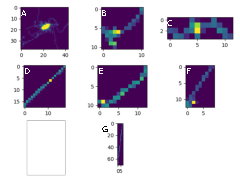
\includegraphics[width=0.8\textwidth]{figures/tracks.pdf}
	\caption{Tracks collected at float.}
	\label{tracks}
	\end{center}
\end{figure}

\begin{figure}[H]
\hfill
\subfigure[LET Spectrum from data collected during the duration of the flight.]{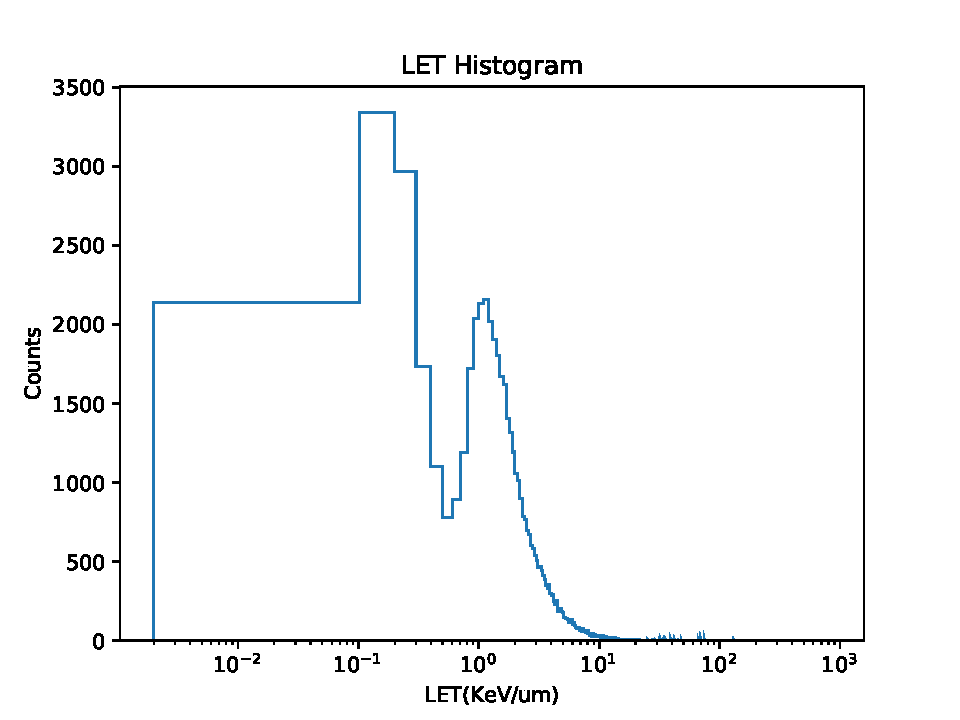
\includegraphics[width=8cm]{figures/LETSpectra2018.pdf}}
\hfill
\subfigure[LET Spectra from each cluster type.]{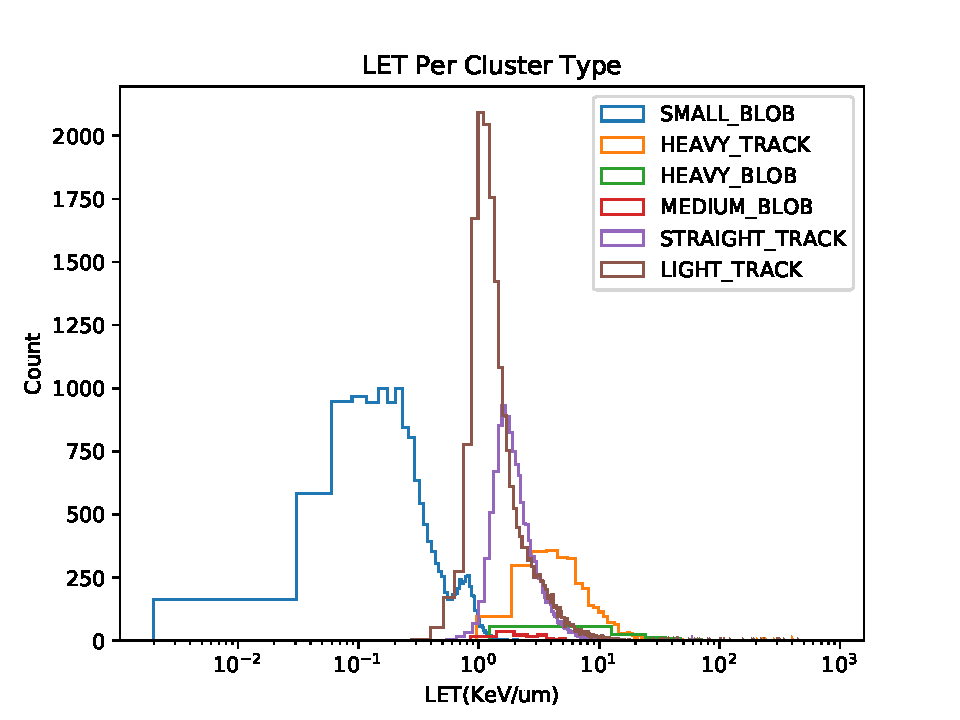
\includegraphics[width=8cm]{figures/LETSpectraPerCluster2018.pdf}}
\hfill
\caption{LET Spectrum data from Flight}
\end{figure}

\begin{figure}[H]
\hfill
\subfigure[LET Spectrum from data collected during the duration of 2017 flight.]{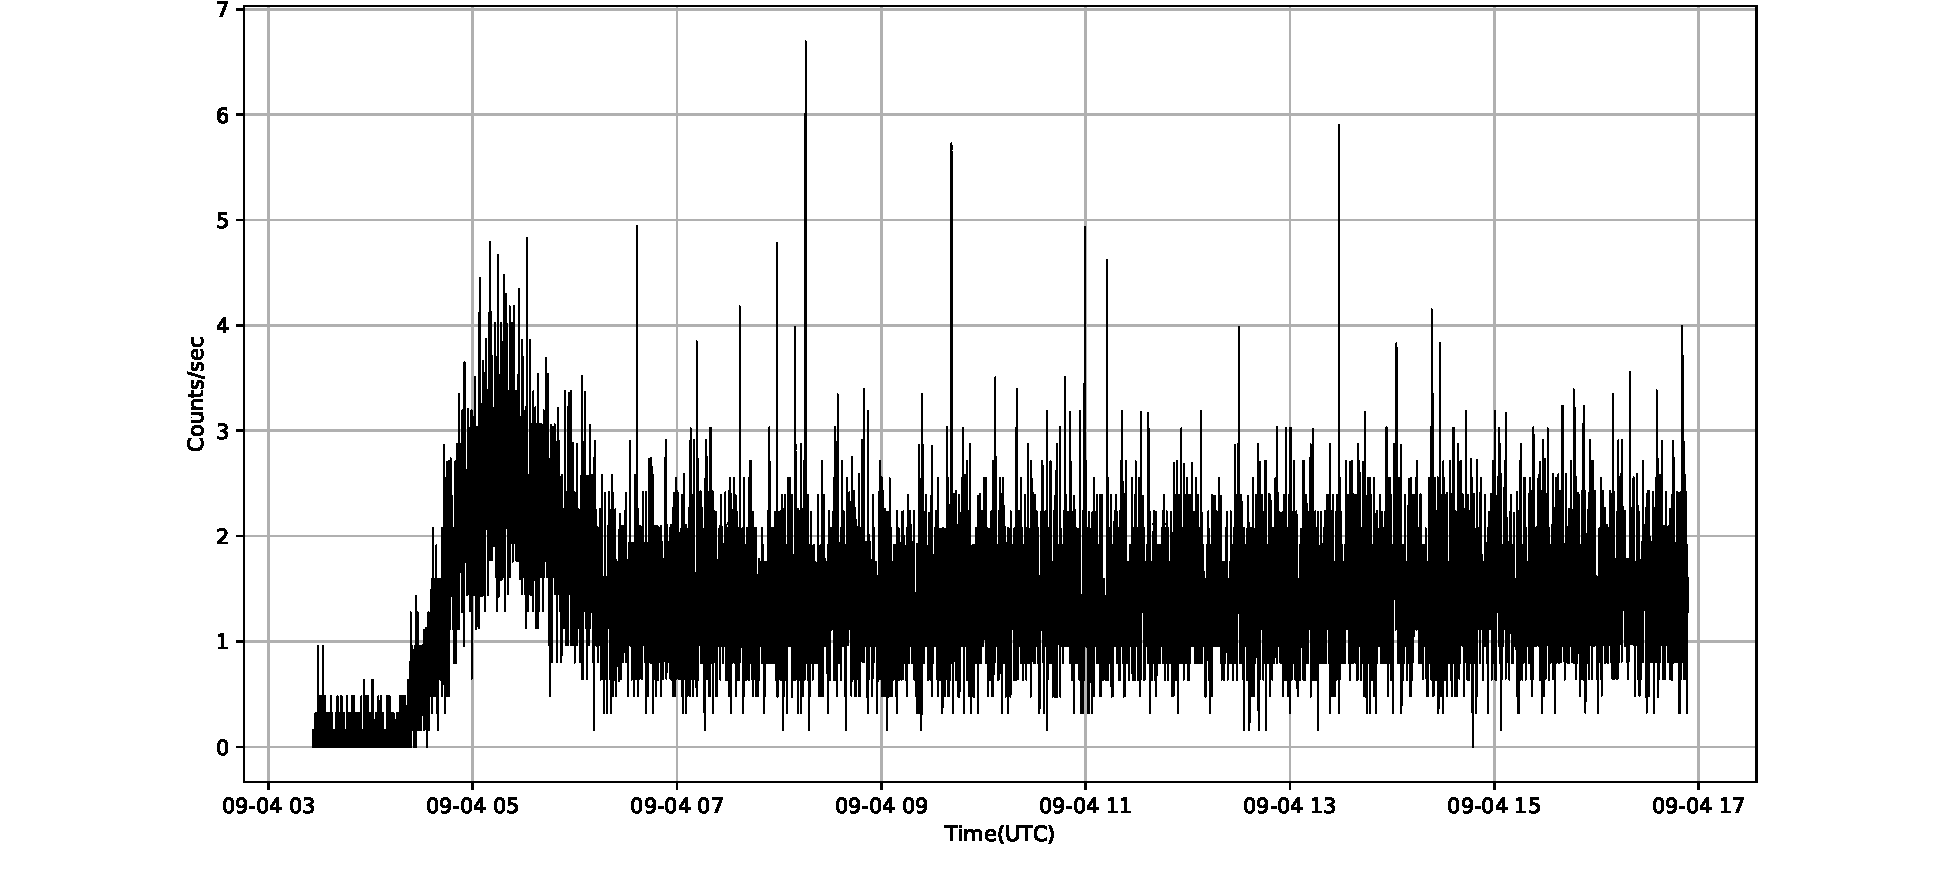
\includegraphics[width=\textwidth]{figures/counts_per_second_2017.pdf}}
\hfill
\subfigure[LET Spectrum from data collected during the duration of 2018 flight.]{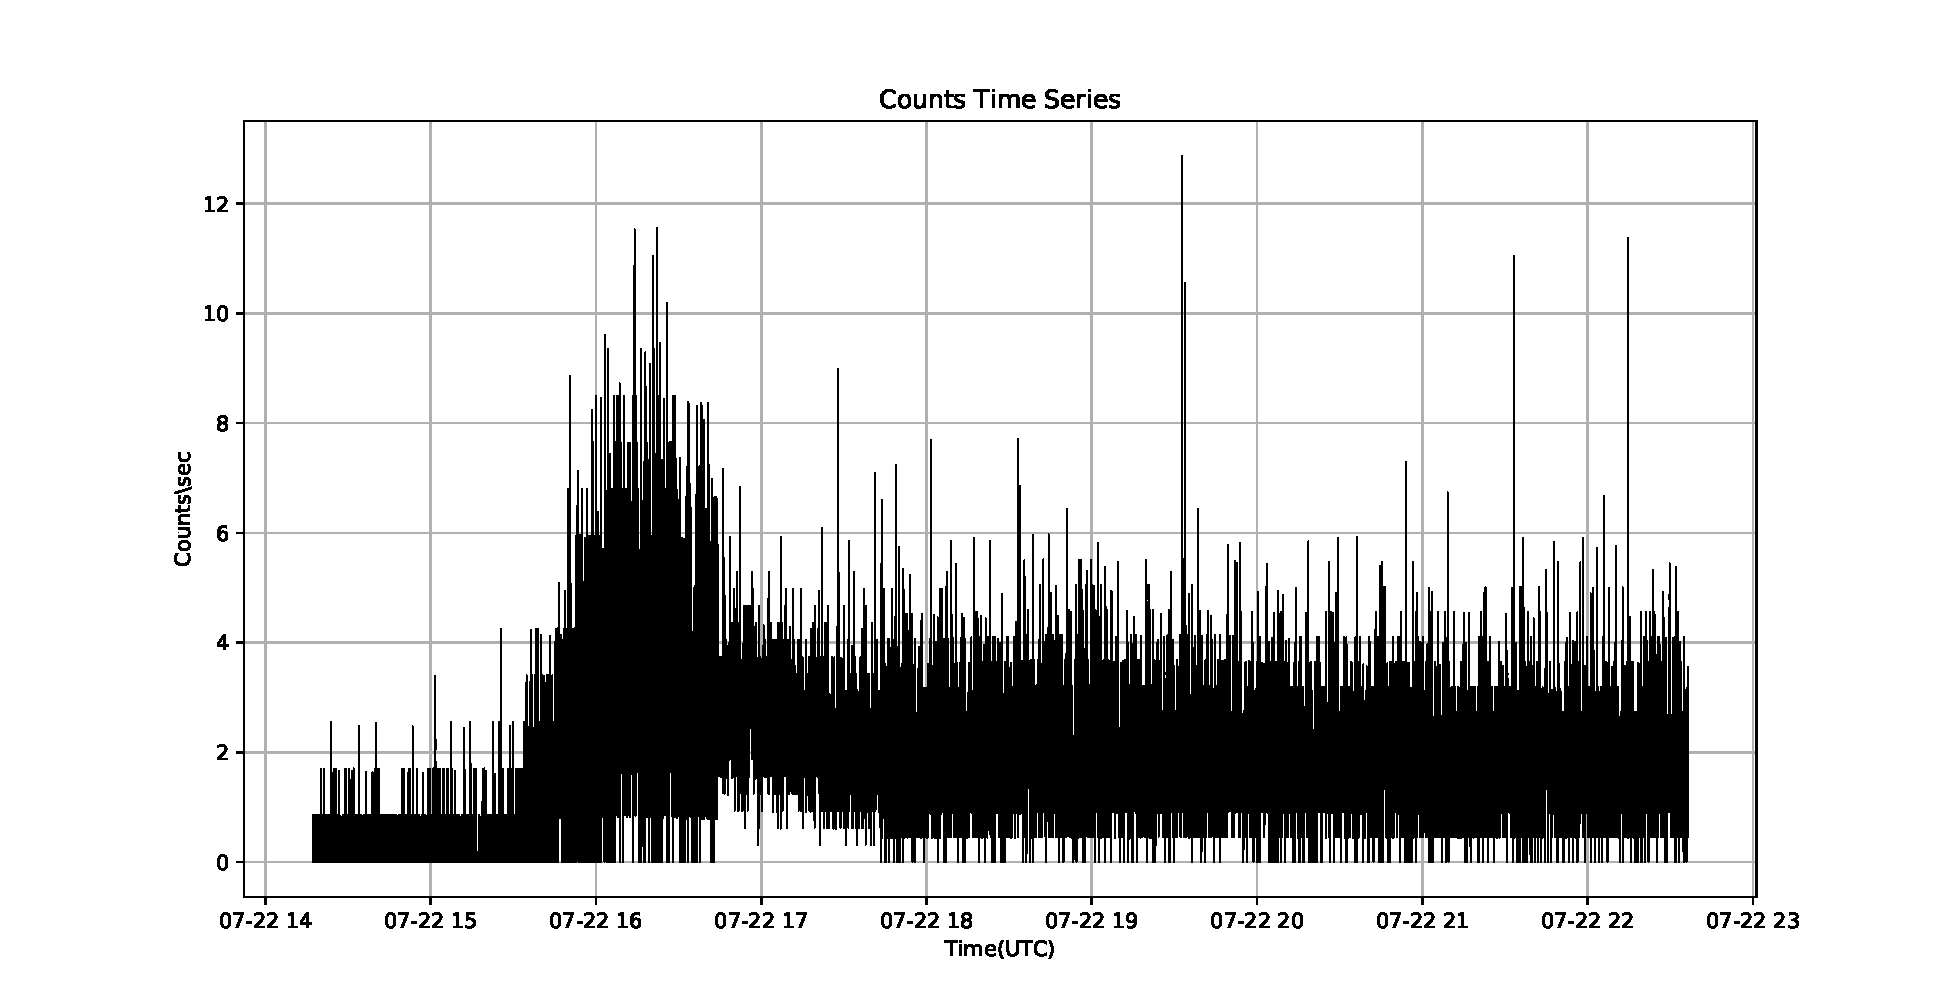
\includegraphics[width=\textwidth]{figures/counts_per_second_2018.pdf}}
\hfill
\caption{LET Spectrum data from Flights 2018 and 2017}
\end{figure}

